\documentclass[12pt,a4paper]{article}

\usepackage{geometry}
\usepackage{longtable}
\usepackage{array}
\usepackage{booktabs}
\usepackage{float}
\usepackage{listings}
\usepackage{xcolor}
\usepackage{hyperref}
\usepackage{pdflscape}
\usepackage{makecell}
\usepackage{tikz}
\usepackage{graphicx}
\usetikzlibrary{arrows.meta,positioning,shapes.geometric}

\usepackage{xepersian}

\geometry{
    top=2.5cm,
    bottom=2.5cm,
    left=2cm,
    right=2cm
}

\settextfont[
    Path=./,
    UprightFont={XB Niloofar.ttf},
    BoldFont={XB NiloofarBd.ttf},
    ItalicFont={XB NiloofarIt.ttf},
    BoldItalicFont={XB NiloofarBdIt.ttf}
]{XB Niloofar}

\setlatintextfont{TeX Gyre Termes}

\renewcommand{\arraystretch}{1.35}
\setlength{\tabcolsep}{4pt}

\newcolumntype{P}[1]{>{\raggedleft\arraybackslash}p{#1}}
\newcolumntype{C}[1]{>{\centering\arraybackslash}p{#1}}

\newcommand{\ep}[1]{\lr{\texttt{#1}}}
\newcommand{\tc}[1]{\lr{\texttt{#1}}}
\newcommand{\api}[1]{\lr{\texttt{\footnotesize #1}}}
\newcommand{\ok}{بله}
\newcommand{\nok}{خیر}
\newcommand{\na}{--}
\newcommand{\smalltable}{\fontsize{8.5}{10}\selectfont}
\newcommand{\en}[1]{\lr{\texttt{\detokenize{#1}}}}
\newcommand{\term}[1]{\lr{#1}}
\newcommand{\reservedbox}[2]{%
    \begin{quote}
    \textbf{#1}\\[0.3em]
    #2
    \end{quote}
}

\definecolor{codegray}{gray}{0.95}

\lstset{
    backgroundcolor=\color{codegray},
    basicstyle=\ttfamily\small,
    breaklines=true,
    frame=single,
    numbers=left,
    numberstyle=\tiny,
    xleftmargin=1em,
    xrightmargin=1em
}

\title{گزارش طراحی و معماری سامانه جامع فروش بلیت رویداد تیکت‌پلاس}
\author{نام اعضای گروه: \underline{\hspace{6cm}}}
\date{\today}

\begin{document}

\maketitle
\tableofcontents
\newpage

\section*{چکیده}
\addcontentsline{toc}{section}{چکیده}

این گزارش طراحی، معماری، زیرساخت، تضمین کیفیت و عملیات سامانه فروش بلیت
«تیکت‌پلاس» را مستند می‌کند. مسئله اصلی سامانه، ارائه تجربه خرید قابل اعتماد
در شرایط هجوم ناگهانی کاربران است؛ شرایطی که در آن کنترل هم‌زمانی، جلوگیری از
رزرو مضاعف، مدیریت نتیجه مبهم پرداخت و آزادسازی خودکار صندلی اهمیت حیاتی دارد.
معماری پیشنهادی بر حوزه‌های مستقل هویت، کاتالوگ، اتاق انتظار، رزرو و موجودی،
پرداخت، صدور بلیت و اعلان استوار است. در محیط تولید از کوبرنتیز، پستگرس، ردیس،
کافکا و زیرساخت کدنویسی‌شده با ترافورم استفاده می‌شود.

علاوه بر مدل‌های معماری، یک پیاده‌سازی مرجع بدون وابستگی خارجی برای جریان
رزرو، پرداخت، جبران، صدور بلیت و اعلان فراهم شده است. آزمون‌های خودکار شامل
رقابت هم‌زمان ۲۰۰ درخواست برای یک صندلی، آزمون مرز انقضا، تکرار امن درخواست و
سناریوهای موفق، ناموفق و مبهم پرداخت است. در اجرای نهایی، ۹ آزمون موفق، پوشش
دستوری ۹۳٫۰۷ درصد در ماژول‌های تراکنشی و امتیاز جهش ۱۰۰ درصد برای شش جهش
حیاتی ثبت شد. بخش‌های چشم‌انداز محصول، تحلیل ریسک و شواهد جیرا عمداً برای درج
نسخه نهایی تهیه‌شده توسط گروه خالی نگه داشته شده‌اند.

\section{معرفی پروژه و اهداف کلان}

تیکت‌پلاس یک سکوی فروش بلیت برای رویدادهای فرهنگی، هنری، ورزشی و تجاری است.
سامانه چرخه‌ای از ایجاد رویداد و تعریف سالن تا جست‌وجو، ورود به اتاق انتظار،
انتخاب صندلی، پرداخت، صدور بلیت دارای کد \term{QR} و ارسال اعلان را پوشش
می‌دهد. ویژگی متمایز سامانه این است که صحت مالکیت صندلی را بر دسترس‌پذیری
ظاهری مقدم می‌داند؛ بنابراین در صورت نامشخص بودن وضعیت، درخواست خرید به شکل
ایمن رد یا در وضعیت نیازمند تطبیق نگهداری می‌شود.

\subsection{اهداف محصول}
\begin{itemize}
  \item جست‌وجوی سریع رویدادها بر اساس دسته، تاریخ، مکان و ظرفیت؛
  \item نمایش نقشه سالن و وضعیت قابل فهم صندلی‌ها؛
  \item تضمین اینکه هر صندلی در هر رویداد حداکثر یک مالک تأییدشده دارد؛
  \item حفظ جایگاه منصفانه کاربران در رویدادهای پرترافیک؛
  \item پردازش امن و تکرارپذیر پرداخت و جبران خودکار شکست‌ها؛
  \item صدور فوری بلیت و ارسال اعلان بدون وابسته کردن پرداخت به سرویس اعلان؛
  \item مقیاس‌پذیری مستقل حوزه‌های پرترافیک و مشاهده‌پذیری کامل عملیات.
\end{itemize}

\subsection{اهداف سازمانی}
اعتماد خریدار و برگزارکننده، دسترس‌پذیری بالا، گزارش لحظه‌ای فروش، توسعه‌پذیری
برای درگاه‌های پرداخت و مشتریان موبایل و کاهش زمان بازیابی رخدادهای تولید،
اهداف سازمانی اصلی هستند. معیار مطلق صحت، صفر بودن رزرو مضاعف تأییدشده است.

\reservedbox{فضای تکمیل مشخصات پروژه}{در این قسمت اعضای گروه می‌توانند نام
دانشگاه، نام و شماره دانشجویی اعضا، نقش هر عضو، تاریخ‌ها و خلاصه تقسیم کار واقعی
را درج کنند.}

\section{نیازمندی‌ها و قابلیت‌های سامانه}

\subsection{قابلیت‌های کارکردی}
\begin{longtable}{P{3.3cm}P{10.8cm}}
\toprule
قابلیت & شرح\\
\midrule
هویت و دسترسی & ثبت‌نام، ورود، توکن کوتاه‌عمر و کنترل نقش خریدار، برگزارکننده و مدیر\\
مدیریت سالن و رویداد & تعریف بخش، ردیف، صندلی، زمان‌بندی، قیمت‌گذاری و وضعیت انتشار\\
کشف رویداد & جست‌وجو و فیلتر بر اساس کلیدواژه، دسته، تاریخ، مکان و برآورد ظرفیت\\
اتاق انتظار & نگهداری جایگاه پایدار، صدور توکن امضاشده و کنترل نرخ پذیرش\\
رزرو صندلی & قفل زمان‌دار، جلوگیری از رقابت مخرب، انقضا و لغو ایمن\\
پرداخت & کلید تکرارپذیری، مدیریت نتیجه قطعی یا مبهم و الگوی ساگا\\
صدور بلیت & ایجاد شناسه و هش \term{QR} پس از تأیید پایدار پرداخت\\
اعلان & ایمیل، پیامک و وضعیت زنده با مصرف رویدادهای غیرهم‌زمان\\
تحلیل برگزارکننده & فروش، درآمد، ظرفیت باقی‌مانده و نرخ تبدیل\\
\bottomrule
\end{longtable}

\subsection{قواعد حیاتی کسب‌وکار}
\begin{enumerate}
  \item وضعیت زنده صندلی تنها توسط حوزه رزرو و موجودی تغییر می‌کند.
  \item تأیید رزرو منقضی یا لغوشده مجاز نیست.
  \item هر درخواست قابل تکرار، کلید \term{Idempotency} پایدار دارد.
  \item timeout درگاه به معنای شکست قطعی نیست و با وضعیت «نامشخص» تطبیق می‌شود.
  \item صدور بلیت فقط پس از رویداد موفقیت پرداخت انجام می‌شود.
  \item تحویل چندباره پیام نباید بلیت، پرداخت یا اعلان کسب‌وکاری تکراری ایجاد کند.
\end{enumerate}

\subsection{اسناد پایه رزروشده}
\reservedbox{چشم‌انداز محصول}{نسخه نهایی سند چشم‌انداز محصول در این قسمت یا
به‌عنوان پیوست مستقل قرار گیرد. سند باید اهداف بلندمدت، پرسوناهای خریدار،
برگزارکننده و مدیر، ارزش پیشنهادی، محدوده و معیارهای کسب‌وکاری را پوشش دهد.}

\reservedbox{تحلیل و کاهش ریسک}{نسخه نهایی تحلیل ریسک گروه در این قسمت قرار
گیرد. سناریوهای ضروری شامل هجوم ناگهانی، خرابی درگاه پرداخت، ناسازگاری داده،
خرابی ردیس، عقب‌ماندگی کافکا و پارتیشن شبکه هستند.}

\section{مدل‌سازی و معماری سامانه}

همه نمودارهای اصلی با \term{PlantUML} نگهداری شده‌اند. منبع متنی نمودارها در
پوشه \en{diagrams/} و خروجی برداری آن‌ها در \en{rendered/} قرار دارد. این روش
بازبینی تغییرات و بازتولید خودکار خروجی در خط لوله را ممکن می‌کند.

\subsection{نمودار موارد کاربرد}
این نمودار بازیگران خریدار، برگزارکننده، مدیر سامانه، درگاه پرداخت و ارائه‌دهنده
اعلان را به جریان‌های کشف رویداد، رزرو، پرداخت، صدور بلیت و مدیریت رویداد متصل
می‌کند.
\begin{figure}[H]
\centering
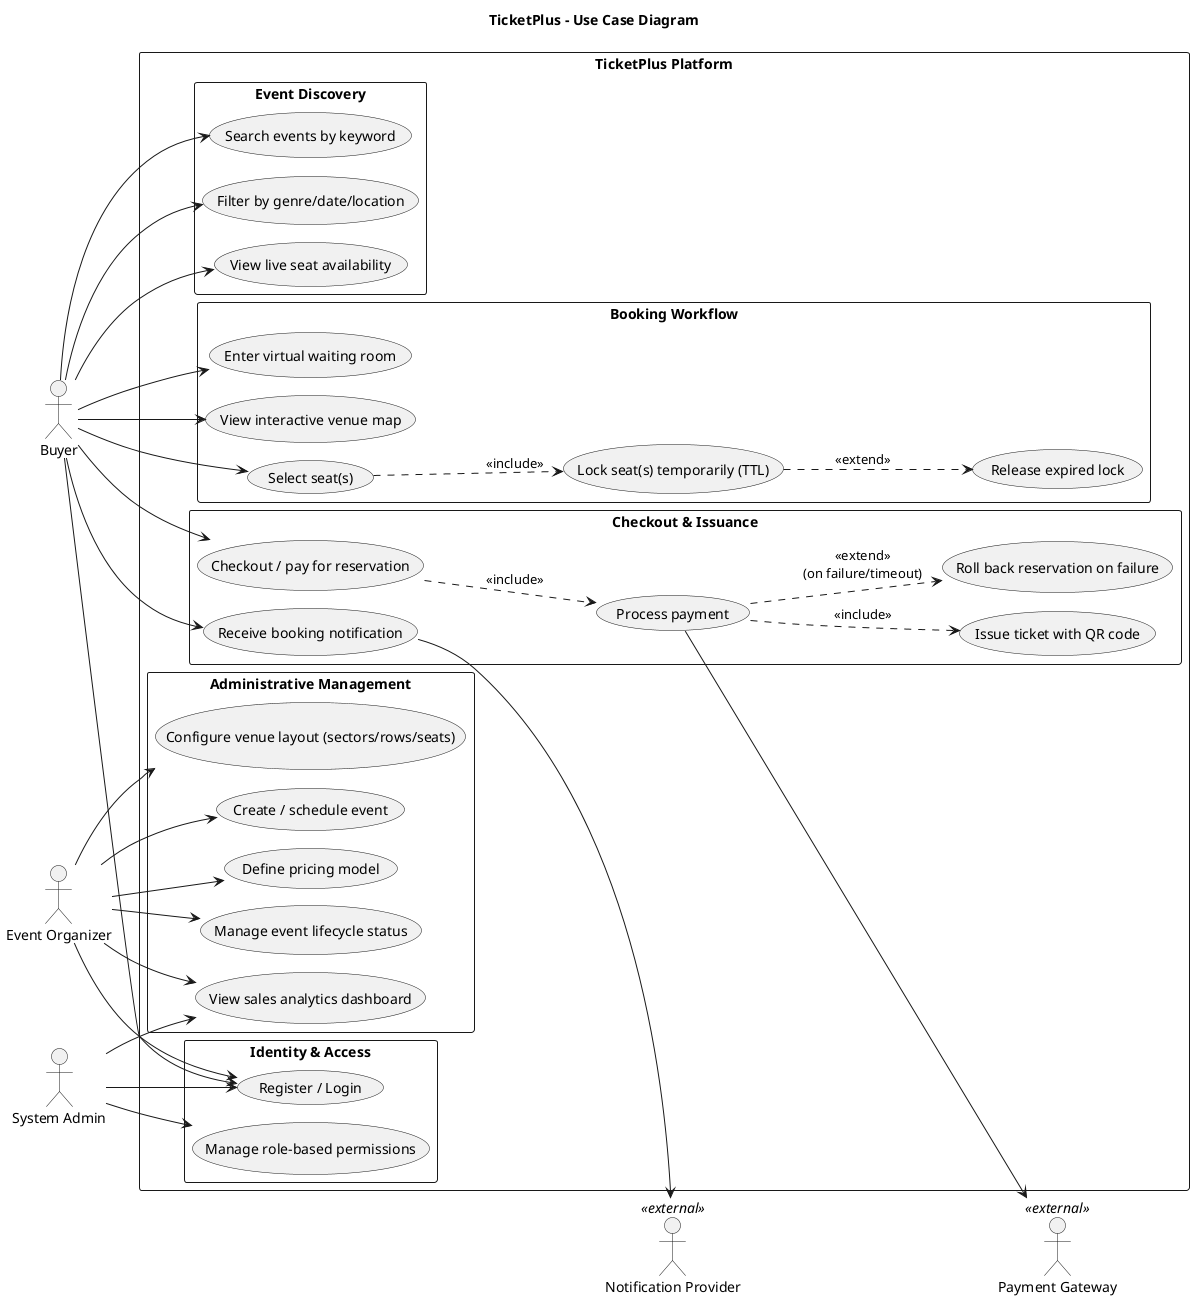
\includegraphics[width=0.94\textwidth,height=0.72\textheight,keepaspectratio]{figures/01-use-case.png}
\caption{نمودار موارد کاربرد تیکت‌پلاس}
\end{figure}

\subsection{نمودار کلاس}
مدل دامنه شامل کاربر، برگزارکننده، رویداد، سالن، بخش، ردیف، صندلی، قانون قیمت،
رزرو، پرداخت، بلیت و اعلان است. وضعیت رزرو و پرداخت صریح مدل شده و زمان انقضا و
کلید تکرارپذیری در موجودیت رزرو قرار دارد.
\begin{figure}[H]
\centering
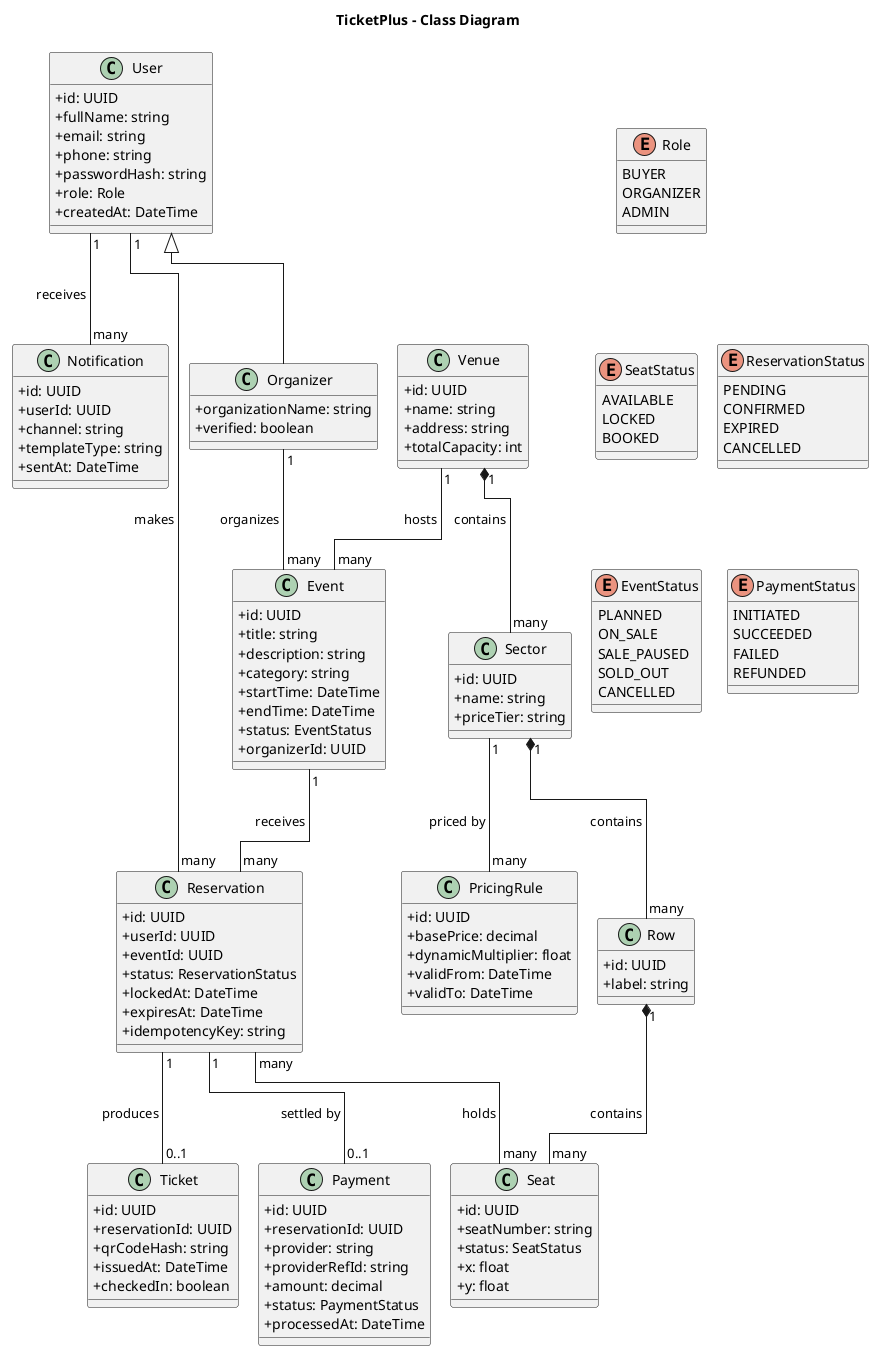
\includegraphics[width=0.96\textwidth,height=0.78\textheight,keepaspectratio]{figures/02-class-diagram.png}
\caption{نمودار کلاس‌های اصلی دامنه}
\end{figure}

\subsection{نمودارهای توالی}
توالی خرید، ورود اختیاری به اتاق انتظار، قفل اتمیک، ثبت رزرو، فراخوانی درگاه،
تأیید یا جبران و صدور مستقل بلیت را نشان می‌دهد. در شکست پرداخت، رزرو لغو و
صندلی آزاد می‌شود. در انقضای بدون پرداخت نیز کلید قفل حذف و وضعیت رزرو منقضی
می‌شود.
\begin{figure}[H]
\centering
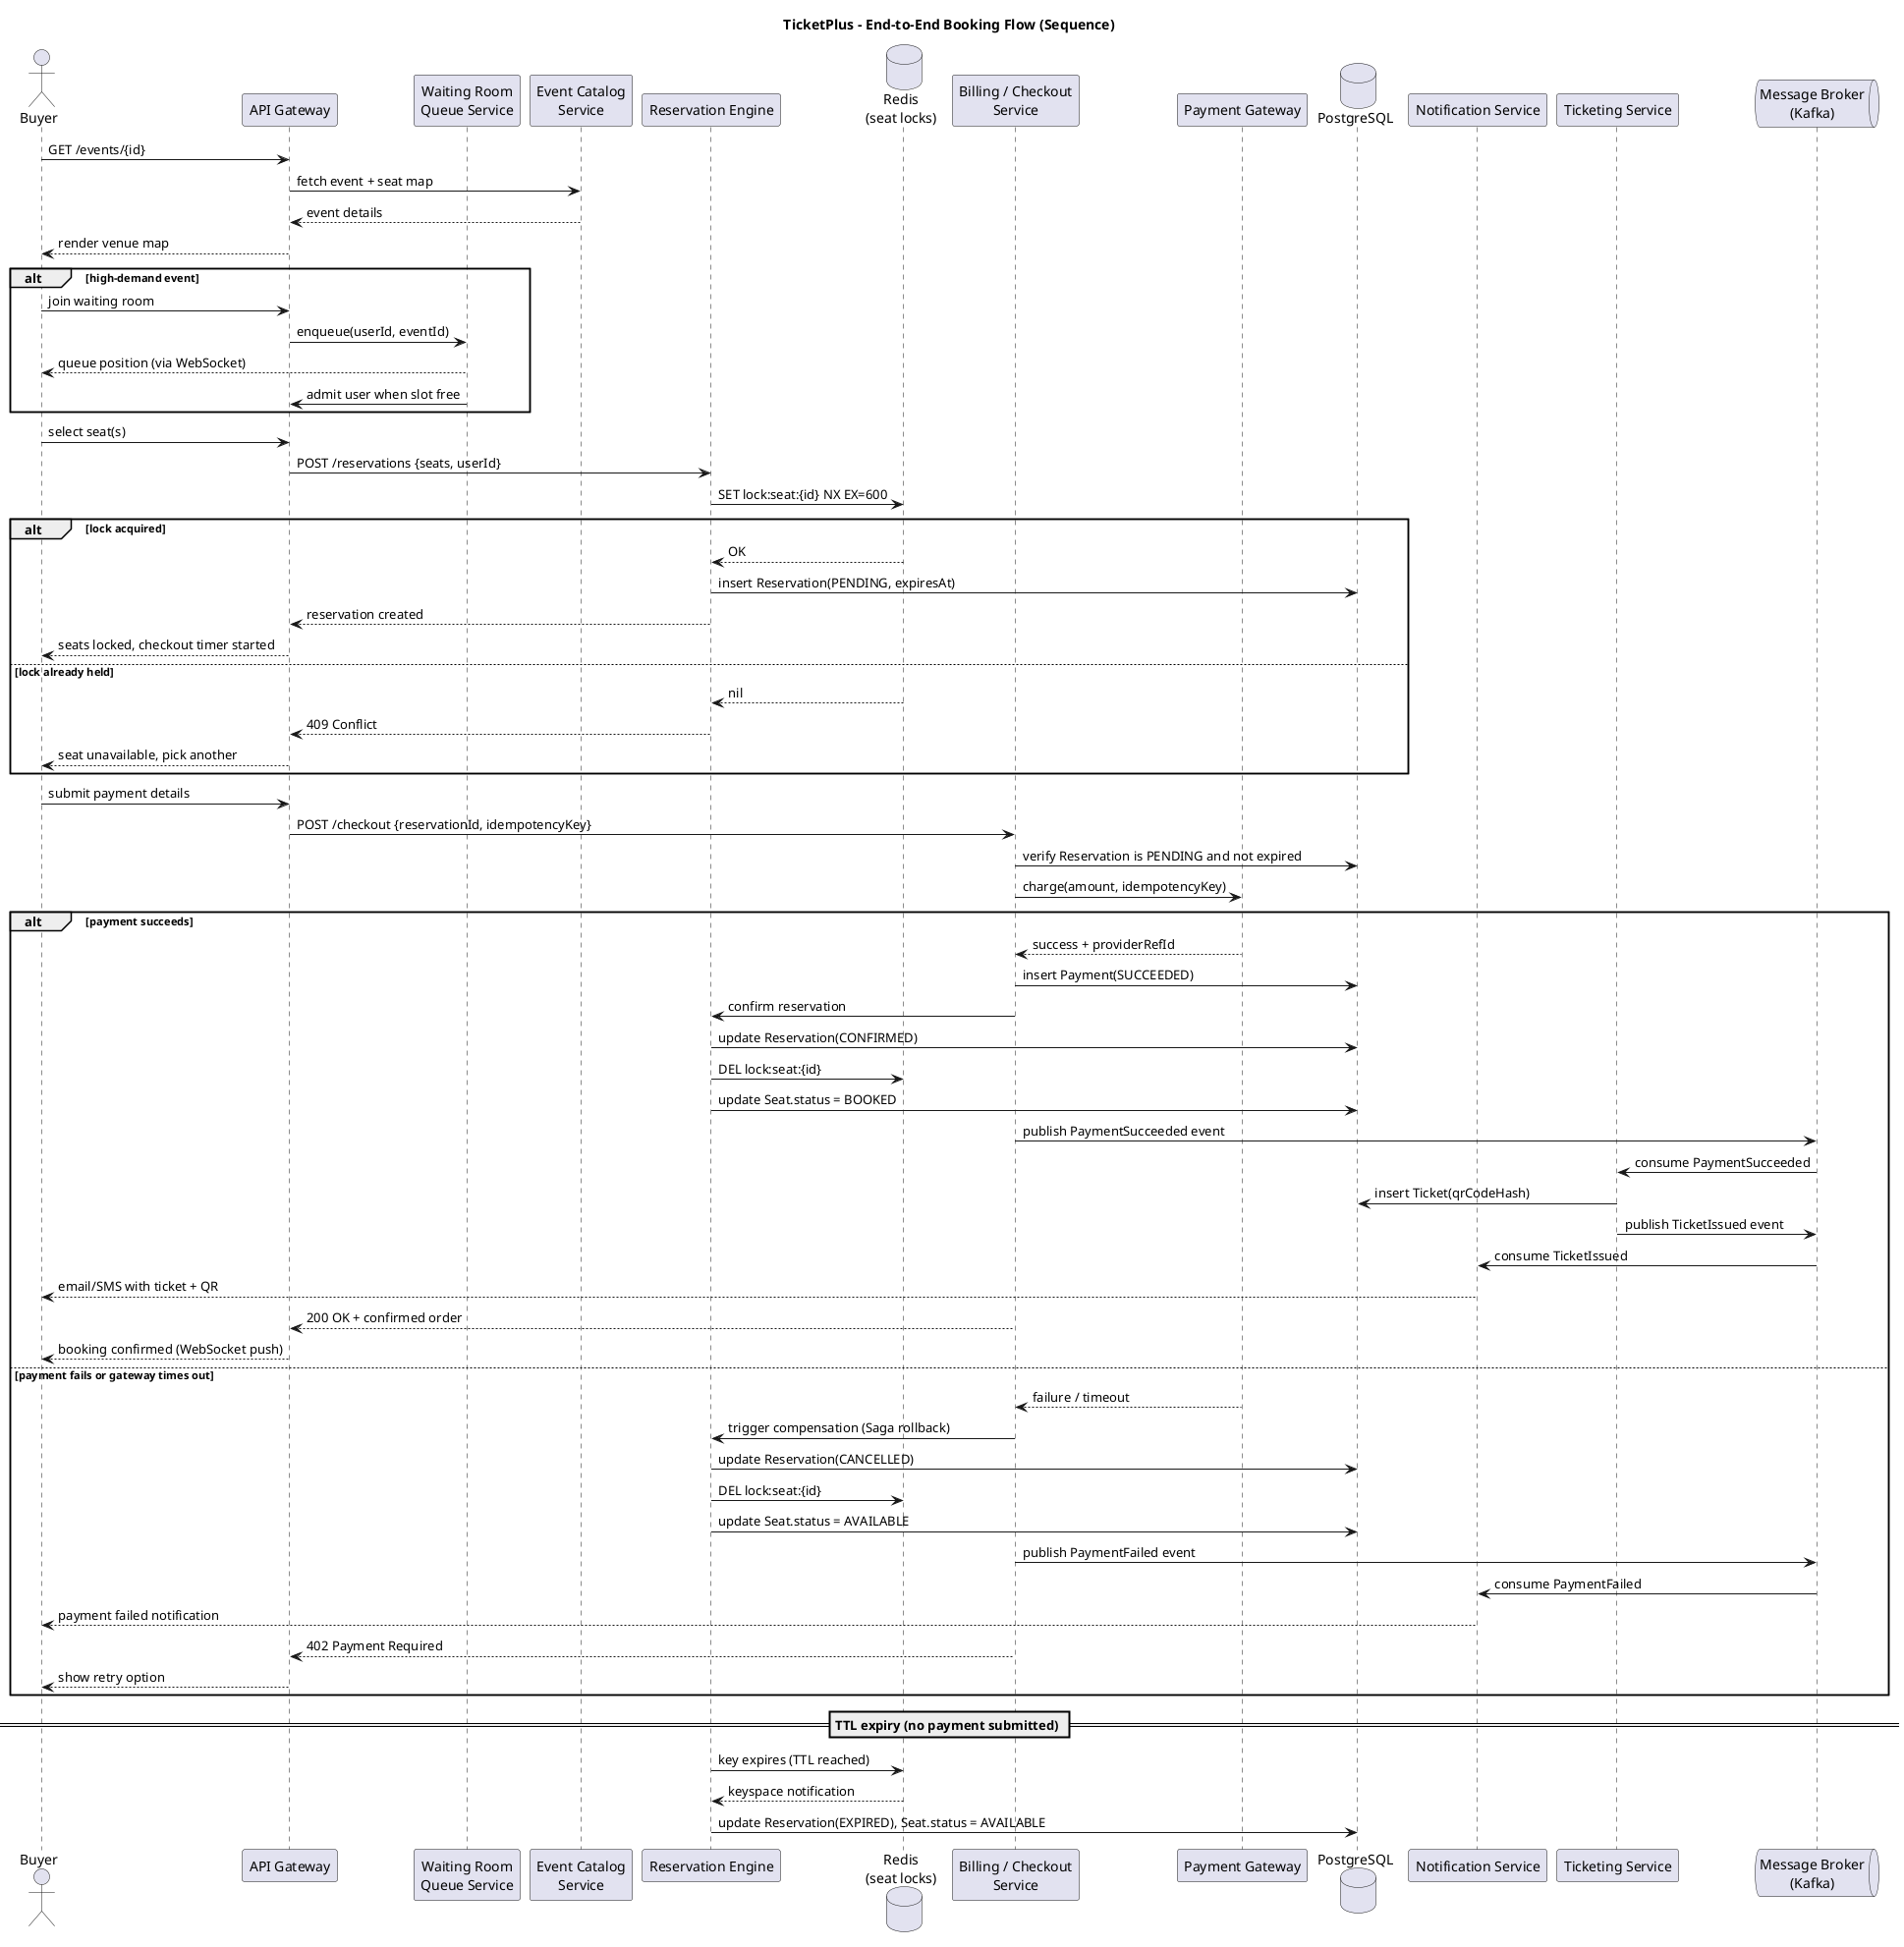
\includegraphics[width=0.96\textwidth,height=0.82\textheight,keepaspectratio]{figures/03-sequence-booking-flow.png}
\caption{توالی انتهابه‌انتهای خرید بلیت}
\end{figure}

جریان اعلان از طریق کافکا از پرداخت جدا شده است. سرویس بلیت رویداد موفقیت
پرداخت را مصرف می‌کند، بلیت را می‌سازد و رویداد صدور بلیت را برای اعلان منتشر
می‌کند.
\begin{figure}[H]
\centering
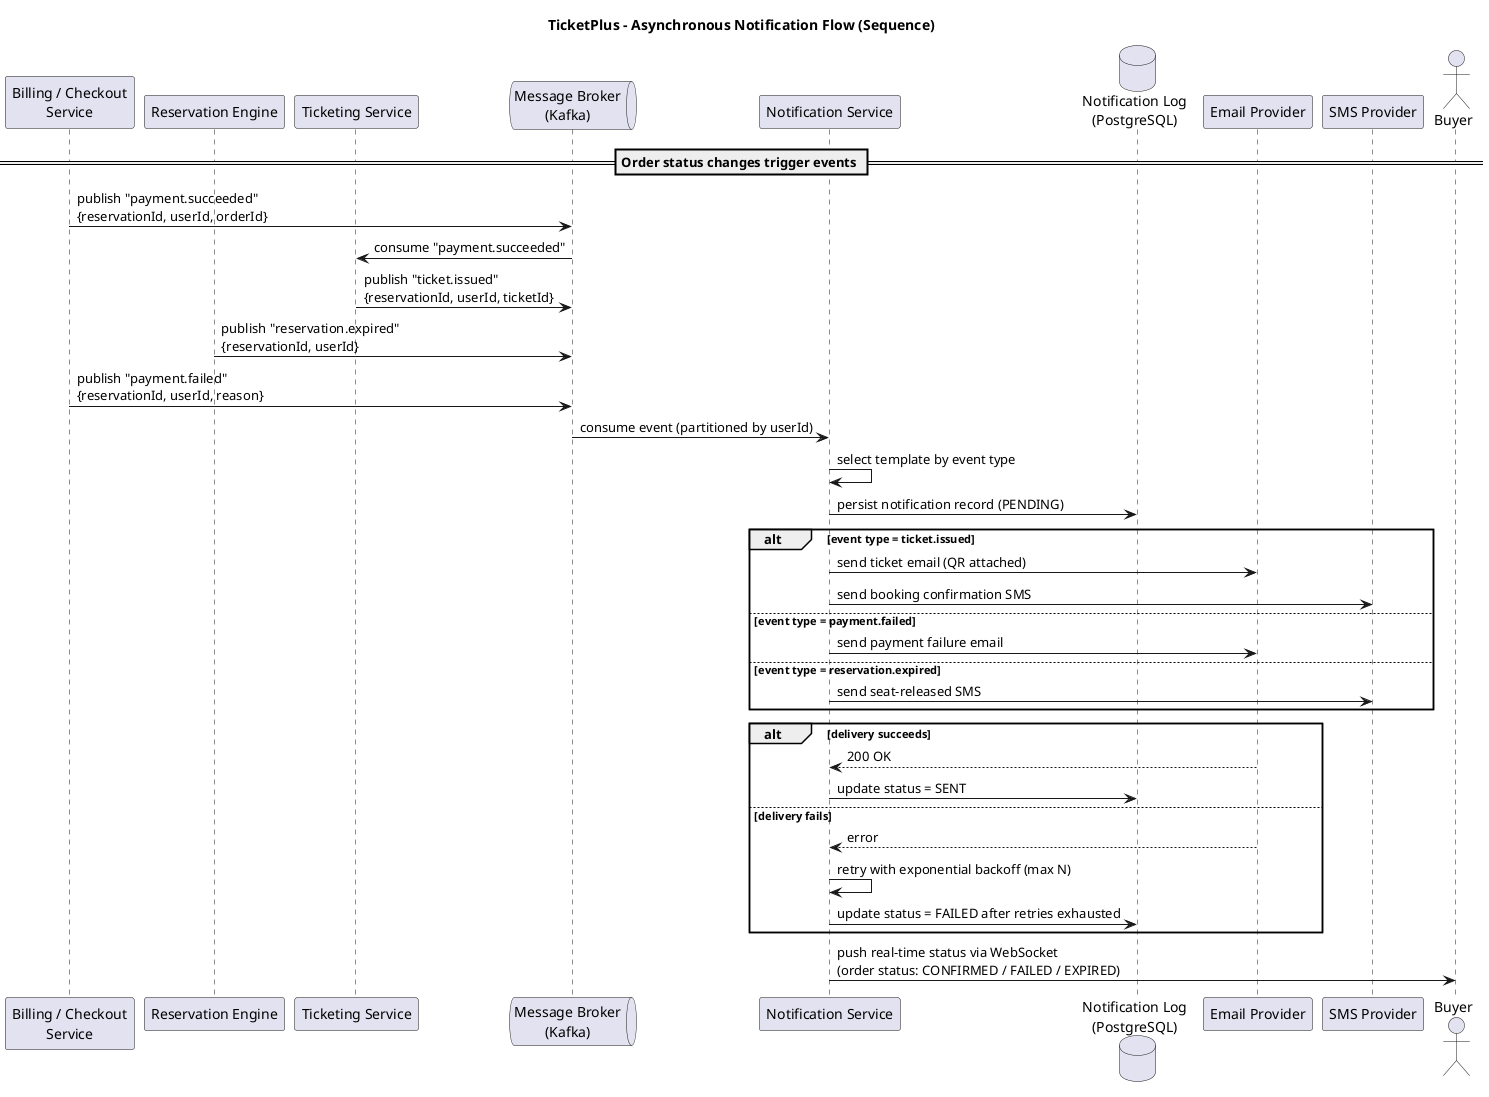
\includegraphics[width=0.95\textwidth,height=0.75\textheight,keepaspectratio]{figures/04-sequence-notification-flow.png}
\caption{توالی اعلان و صدور غیرهم‌زمان بلیت}
\end{figure}

\subsection{نمودارهای فعالیت}
مسیر فعالیت خریدار، شاخه‌های رقابت صندلی، انقضای زمان، شکست پرداخت و خرید موفق
را پوشش می‌دهد. فعالیت برگزارکننده نیز ایجاد سالن، تعریف قیمت، اعتبارسنجی،
انتشار و پایش فروش را مدل می‌کند.
\begin{figure}[H]
\centering
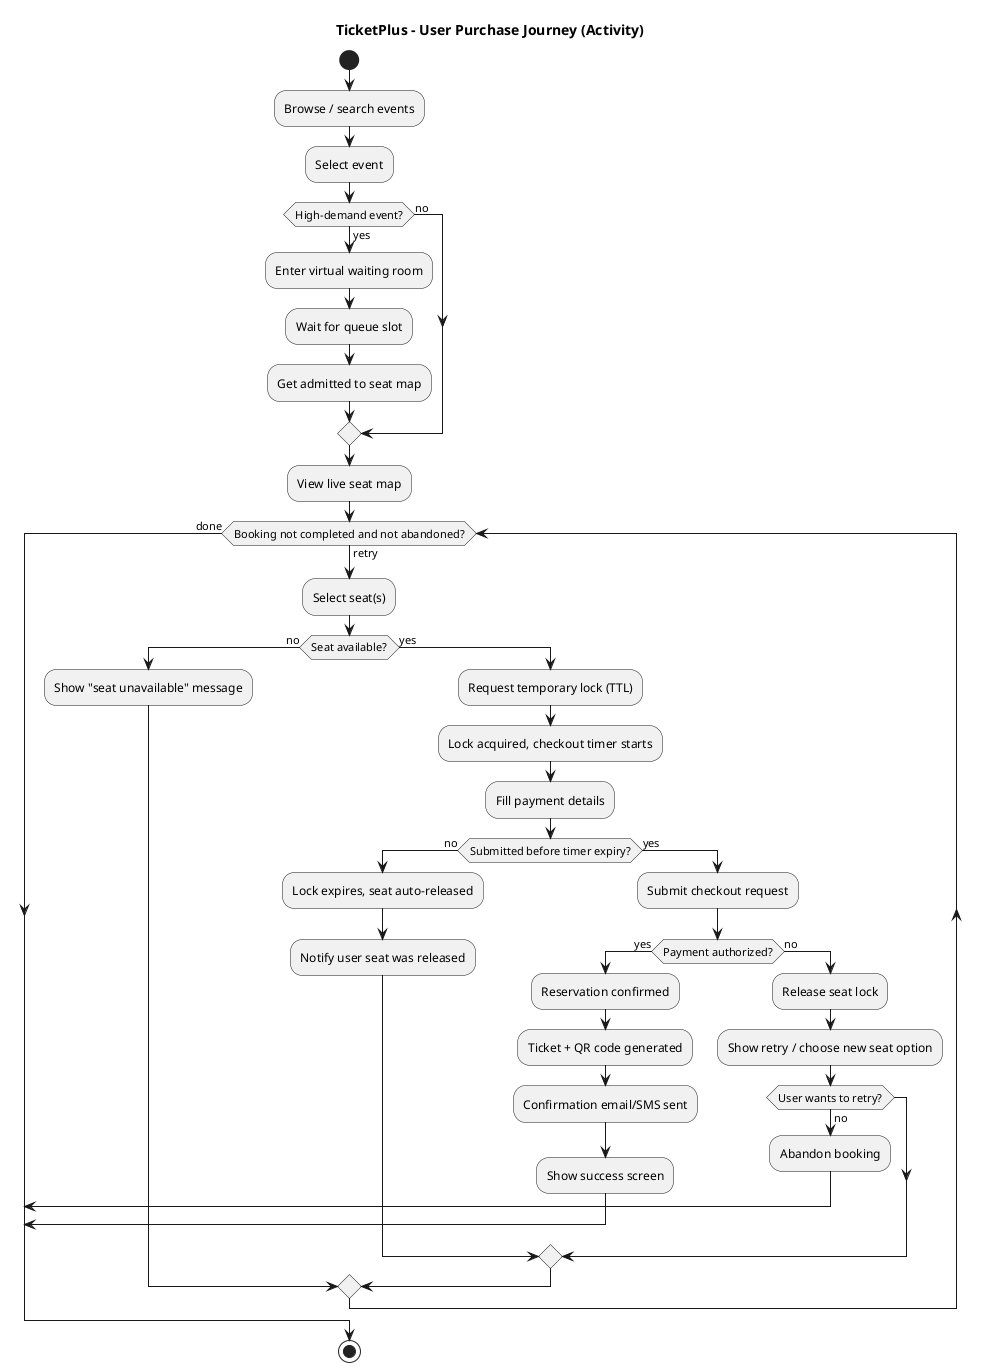
\includegraphics[width=0.88\textwidth,height=0.72\textheight,keepaspectratio]{figures/05-activity-user-purchase.png}
\caption{فعالیت خرید کاربر}
\end{figure}
\begin{figure}[H]
\centering
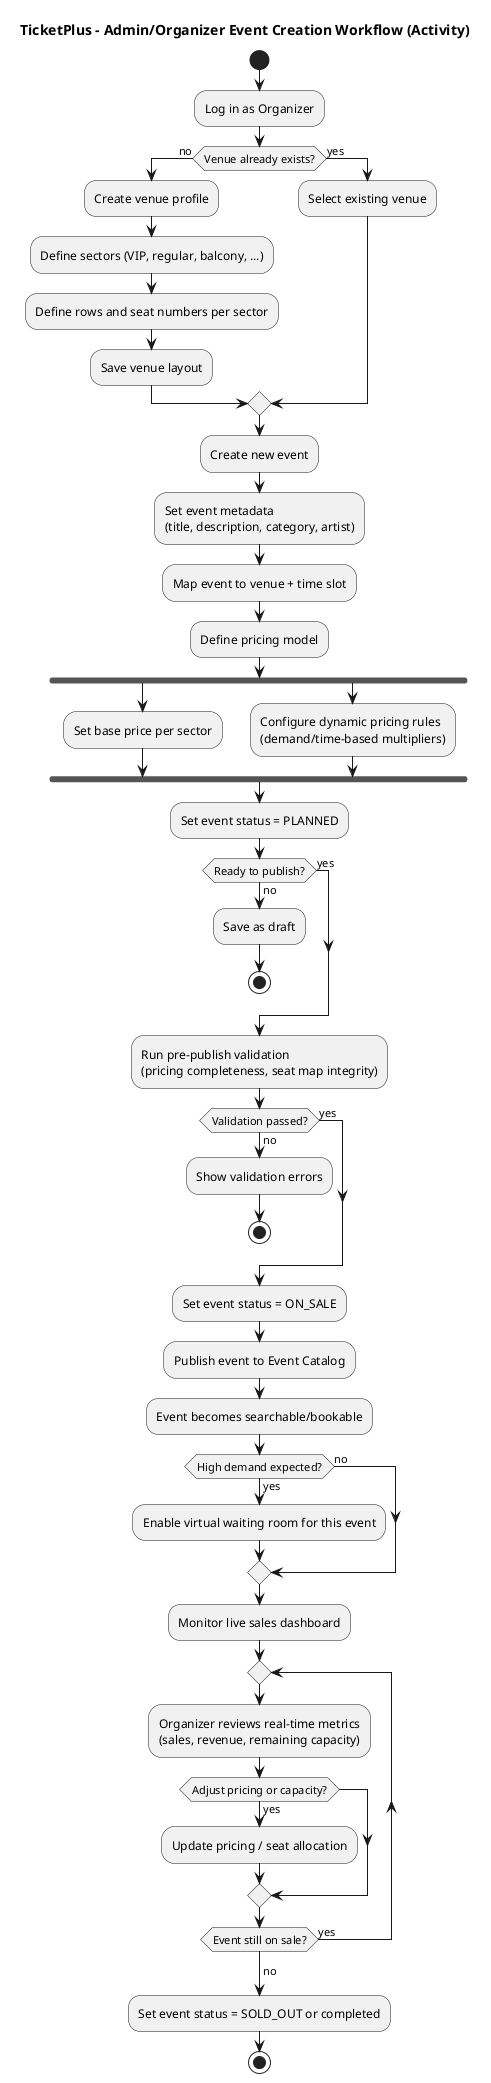
\includegraphics[width=0.88\textwidth,height=0.72\textheight,keepaspectratio]{figures/06-activity-admin-event-creation.png}
\caption{فعالیت ایجاد و انتشار رویداد}
\end{figure}

\subsection{معماری مؤلفه‌ای}
مرزهای مستقل شامل درگاه API، هویت، کاتالوگ، اتاق انتظار، رزرو، پرداخت، بلیت و
اعلان هستند. پایگاه داده هر حوزه به صورت منطقی خصوصی است. سرویس بلیت مالک چرخه
صدور و اعتبارسنجی است و دیگر در حوزه پرداخت قرار ندارد.
\begin{figure}[H]
\centering
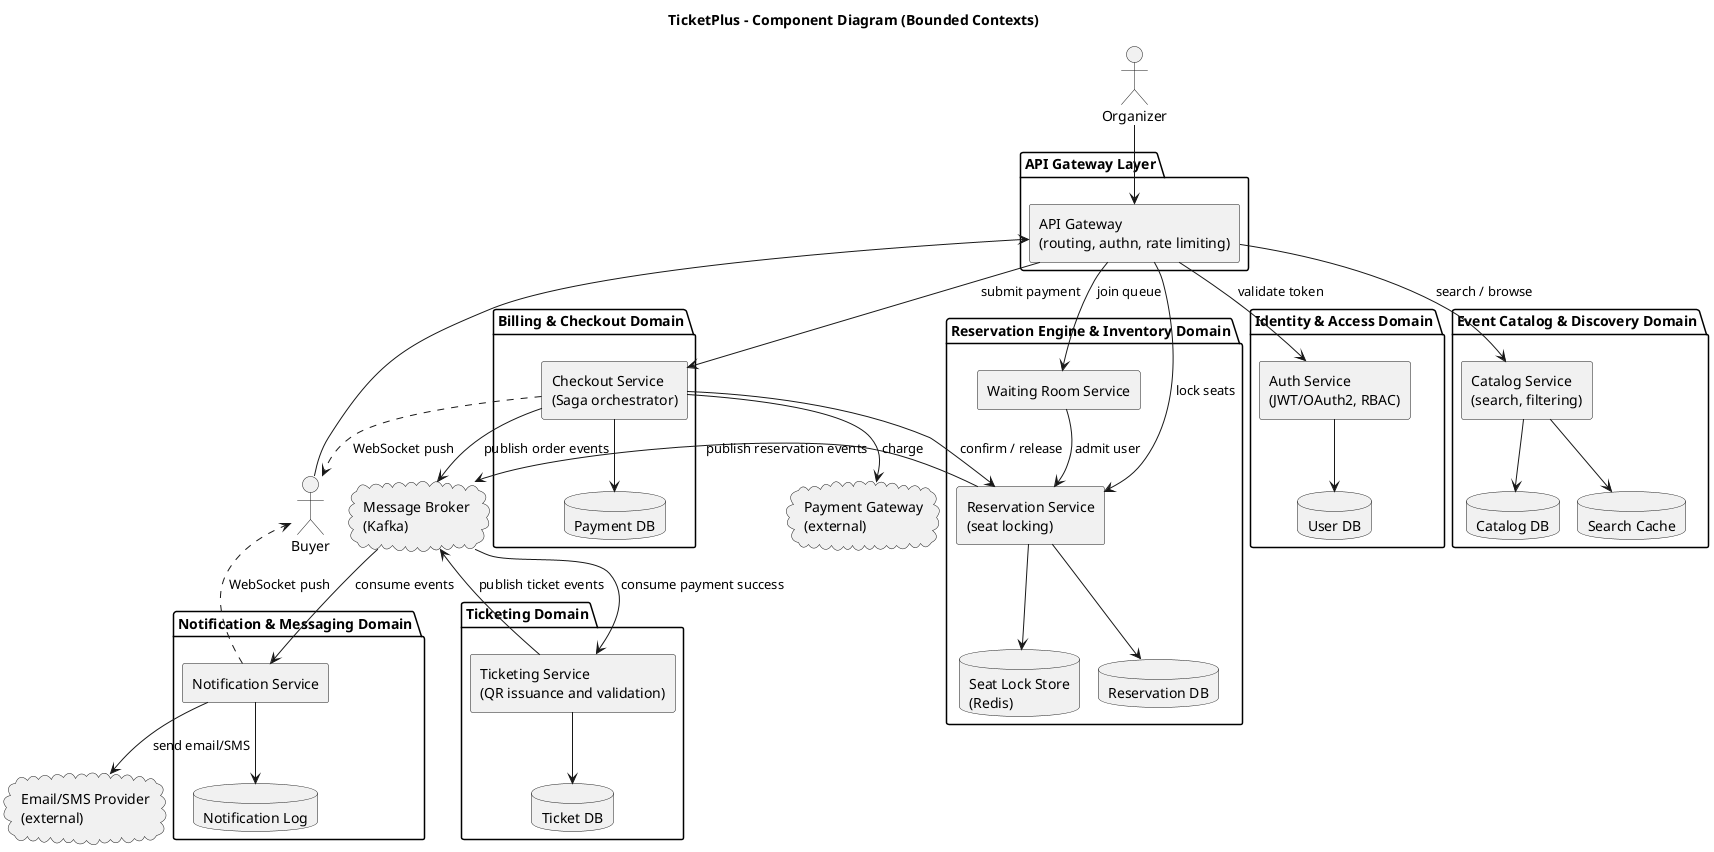
\includegraphics[width=0.98\textwidth,height=0.78\textheight,keepaspectratio]{figures/07-component-diagram.png}
\caption{نمودار مؤلفه‌ها و حوزه‌های سامانه}
\end{figure}

\subsection{معماری استقرار}
در استقرار تولید، ترافیک از بارمتوازن‌کننده و ورودی کوبرنتیز به درگاه API و
سپس سرویس‌ها هدایت می‌شود. پستگرس داده پایدار، ردیس قفل موقت و کافکا رویدادهای
غیرهم‌زمان را نگهداری می‌کنند. پرومتئوس و گرافانا برای پایش استفاده می‌شوند.
\begin{figure}[H]
\centering
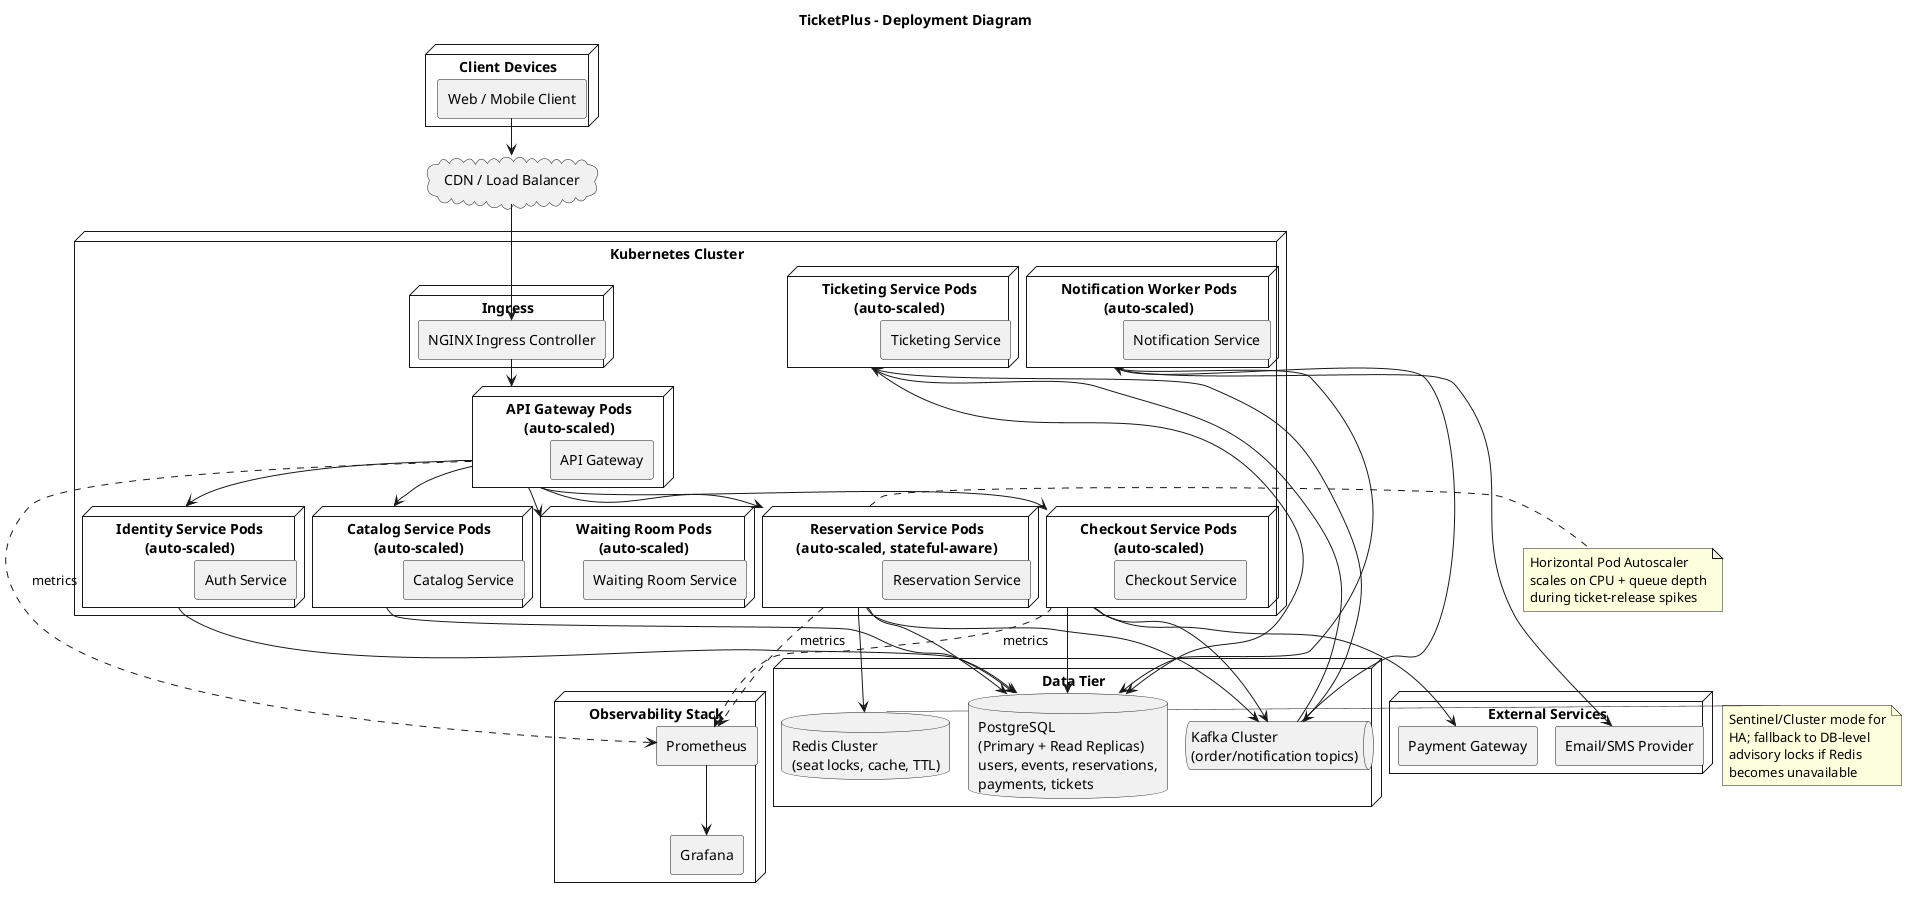
\includegraphics[width=0.98\textwidth,height=0.80\textheight,keepaspectratio]{figures/08-deployment-diagram.png}
\caption{نمودار استقرار تولید}
\end{figure}

\section{زیرساخت و استقرار خودکار}

زیرساخت ابری به صورت اعلامی در \en{infra/terraform/} تعریف شده است. منابع اصلی
عبارت‌اند از شبکه چندناحیه‌ای، زیرشبکه عمومی و خصوصی، دروازه اینترنت، دروازه
\term{NAT}، خوشه \term{EKS}، گروه گره خودمقیاس، پایگاه داده \term{RDS
PostgreSQL} چندناحیه‌ای، ردیس مدیریت‌شده، کافکای مدیریت‌شده \term{MSK} و
بارمتوازن‌کننده کاربردی.

\begin{longtable}{P{4cm}P{10cm}}
\toprule
فایل & مسئولیت\\
\midrule
\en{network.tf} & شبکه، زیرشبکه‌ها، مسیرها و دروازه‌های خروجی\\
\en{eks.tf} & خوشه کوبرنتیز و گروه گره خودمقیاس\\
\en{rds.tf} & پستگرس رمزگذاری‌شده، چندناحیه‌ای و نسخه خواندنی\\
\en{redis.tf} & قفل صندلی با تکرار، failover و رمزگذاری\\
\en{msk.tf} & کارگزاران کافکا، TLS و ثبت رخداد در CloudWatch\\
\en{loadbalancer.tf} & ALB عمومی، listener و target group ورودی\\
\en{variables.tf} و \en{outputs.tf} & پارامترهای محیط و خروجی‌های اتصال\\
\bottomrule
\end{longtable}

فرمت ترافورم با نسخه ۱٫۹٫۸ بررسی شد و اعمال منابع انجام نشد تا هزینه ابری
ایجاد نشود. اعتبارسنجی وابسته به provider در خط لوله گیت‌لب انجام می‌شود؛
registry محلی محیط فعلی پروتکل provider را ارائه نکرد.

\section{چرخه چابک، بازبینی و تضمین کیفیت}

\subsection{فرآیند توسعه و بازبینی}
قواعد مشارکت در \en{CONTRIBUTING.md} تعریف شده است. تغییرات با شاخه مرتبط با
شماره کار جیرا، merge request، آزمون، مستندات و تأیید مالک حوزه ادغام می‌شوند.
تغییرات رزرو، پرداخت، هویت، مهاجرت داده و زیرساخت به دو تأیید نیاز دارند. قالب
merge request شامل رفتار، شواهد آزمون، سازگاری قرارداد، مهاجرت، مشاهده‌پذیری و
روش rollback است.

\subsection{بخش رزروشده مدیریت چابک}
\reservedbox{خروجی جیرا و اسپرینت‌ها}{تصاویر یا خروجی‌های backlog، epic، story،
task، برنامه‌ریزی اسپرینت، burndown chart، sprint review و retrospective واقعی
گروه در این قسمت قرار گیرد. برای هر تصویر شماره اسپرینت و بازه زمانی نوشته شود.}

\reservedbox{شواهد بازبینی کد}{در صورت نیاز، نمونه merge request، نظرهای
بازبین‌ها، نتیجه pipeline و تصمیم ادغام واقعی گروه در این قسمت افزوده شود.}

\subsection{راهبرد آزمون}
اولویت آزمون ابتدا صحت خرید، سپس دسترس‌پذیری، امنیت، کارایی و نگهداشت‌پذیری
است. برای ماژول رزرو حداقل پوشش خط ۹۰ درصد و شاخه ۸۵ درصد و برای منطق حیاتی
امتیاز جهش حداقل ۸۵ درصد تعیین شد. هیچ استثنایی برای رزرو مضاعف، پرداخت تکراری،
دور زدن مجوز یا از دست رفتن غیرقابل بازیابی داده پذیرفته نمی‌شود.

اوراکل صحت پس از آزمون هم‌زمانی بررسی می‌کند که هر صندلی رویداد حداکثر یک رزرو
تأییدشده داشته باشد، هر صندلی فروخته‌شده دقیقاً یک مالک داشته باشد، پرداخت موفق
به سفارش تأییدشده یا بازپرداخت صریح متصل باشد و رزرو منقضی قفل زنده باقی
نگذارد.

\subsection{آزمون‌های پیاده‌سازی‌شده}
پیاده‌سازی مرجع با چارچوب استاندارد \term{unittest} آزموده شد و به نصب بسته
خارجی نیاز ندارد.

\begin{longtable}{P{7.5cm}C{2.2cm}P{4.2cm}}
\toprule
سناریو & وضعیت & نتیجه\\
\midrule
رقابت ۲۰۰ درخواست هم‌زمان برای یک صندلی & موفق & دقیقاً یک برنده\\
تکرار درخواست رزرو با کلید یکسان & موفق & شناسه رزرو یکسان\\
ورودی دارای صندلی تکراری & موفق & رد ورودی\\
انقضا و رزرو مجدد صندلی & موفق & آزادسازی صحیح\\
تأیید دقیقاً در مرز انقضا & موفق & رد و ثبت انقضا\\
پرداخت موفق و صدور بلیت & موفق & تأیید رزرو و یک بلیت\\
پرداخت شکست‌خورده & موفق & جبران و آزادسازی\\
پرداخت با نتیجه نامشخص & موفق & نگهداری برای تطبیق\\
تحویل تکراری رویداد پرداخت & موفق & عدم صدور بلیت دوم\\
آزمون HTTP انتهابه‌انتها & مشروط & در sandbox به علت منع socket رد شد؛ در CI اجرا می‌شود\\
\bottomrule
\end{longtable}

\subsection{پوشش و آزمون جهش}
ابزار پوشش مستقل پروژه، دستورات قابل اجرای ماژول‌های رزرو، پرداخت و رویداد را
با AST پایتون و trace زمان اجرا مقایسه می‌کند. نتیجه آخرین اجرا در جدول زیر است.

\begin{longtable}{P{5cm}C{3cm}C{3cm}C{2.5cm}}
\toprule
ماژول & دستورات قابل اجرا & دستورات پوشش‌یافته & درصد\\
\midrule
\en{reservation.py} & ۱۰۸ & ۹۶ & ۸۸٫۸۹\\
\en{checkout.py} & ۶۱ & ۶۰ & ۹۸٫۳۶\\
\en{events.py} & ۳۳ & ۳۲ & ۹۶٫۹۷\\
مجموع & ۲۰۲ & ۱۸۸ & ۹۳٫۰۷\\
\bottomrule
\end{longtable}

شش جهش حیاتی شامل پذیرش صندلی تکراری، حذف یکتایی مالک فعال، مجاز کردن تأیید در
مرز انقضا، وارونگی موفقیت پرداخت، حذف جبران شکست و حذف تکرارناپذیری صدور بلیت
اعمال شد. همه شش جهش توسط آزمون‌ها کشته شدند و امتیاز جهش ۱۰۰ درصد به دست آمد.

\subsection{آزمون بار و تنش}
اسکریپت \en{quality/load/hot-seat-contention.js} با \term{k6} به طور پیش‌فرض
۵۰۰۰ کاربر مجازی را برای قفل یک صندلی رقابت می‌دهد. معیار پذیرش دقیقاً یک پاسخ
موفق، conflictهای مورد انتظار، خطای فنی کمتر از یک درصد و صدک ۹۵ کمتر از ۷۵۰
میلی‌ثانیه است. برنامه کامل آزمون شامل هجوم لحظه‌ای، بار گسترده رزرو، اوج
پرداخت، soak هشت‌ساعته، spike و تزریق خرابی ردیس، کافکا، درگاه و شبکه است.

\subsection{خط لوله گیت‌لب}
خط لوله \en{.gitlab-ci.yml} مراحل زیر را اجرا می‌کند:
\begin{itemize}
  \item بررسی Markdown و لینک‌ها؛
  \item اعتبارسنجی و بازتولید PlantUML؛
  \item فرمت، init و validate ترافورم بدون backend؛
  \item آزمون، پوشش و جهش پیاده‌سازی مرجع؛
  \item اسکن آسیب‌پذیری، secret و misconfiguration با Trivy؛
  \item اجرای اختیاری آزمون k6 در محیط ایزوله؛
  \item ایجاد فایل ZIP در tag انتشار.
\end{itemize}

\section{معماری تولید و عملیات}

\subsection{مرزبندی حوزه‌ها}
تصمیم اصلی طراحی این است که هندسه سالن در کاتالوگ، اما وضعیت زنده صندلی در
رزرو نگهداری شود. کاتالوگ فقط projection موجودی را برای جست‌وجو مصرف می‌کند و
هرگز وضعیت قفل را نمی‌نویسد. این تصمیم وابستگی حلقوی کاتالوگ و رزرو را حذف و
قاعده جلوگیری از overbooking را به یک مالک واگذار می‌کند.
\begin{figure}[H]
\centering
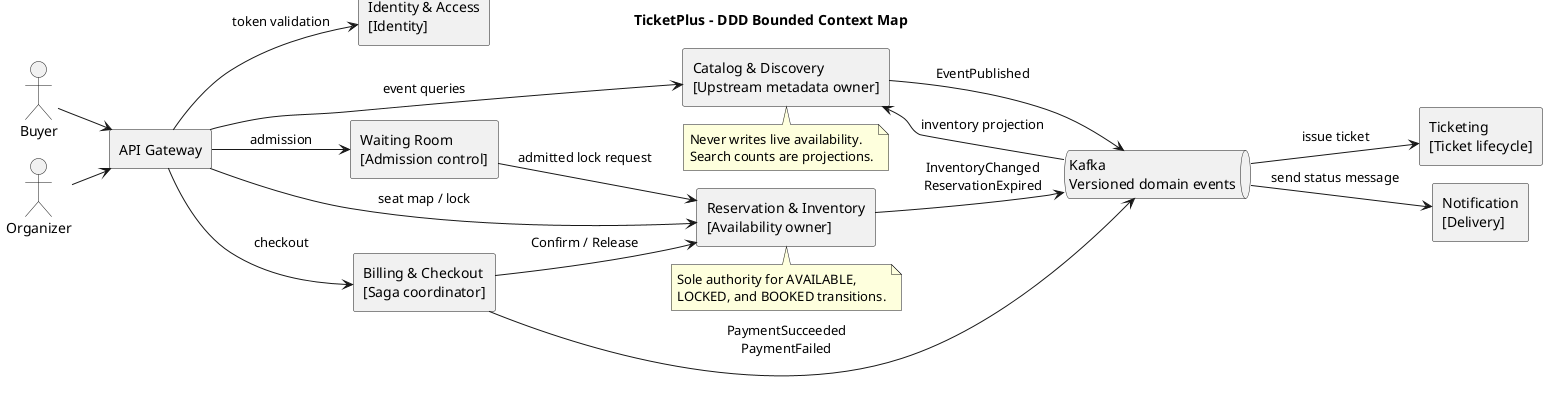
\includegraphics[width=0.96\textwidth,height=0.72\textheight,keepaspectratio]{figures/bounded-context-map.png}
\caption{نقشه حوزه‌های محدودشده}
\end{figure}

\subsection{پیام‌رسانی غیرهم‌زمان}
تغییر وضعیت کسب‌وکار همراه رکورد outbox در یک تراکنش ثبت می‌شود. relay رویداد
را در کافکا منتشر می‌کند. مصرف‌کنندگان شناسه رویداد پردازش‌شده را نگه می‌دارند،
در خطای موقت با backoff و jitter تکرار می‌کنند و پس از پنج شکست پیام را به
dead-letter queue انتقال می‌دهند. کلید پارتیشن شناسه رزرو یا سفارش است تا ترتیب
همان aggregate حفظ شود.
\begin{figure}[H]
\centering
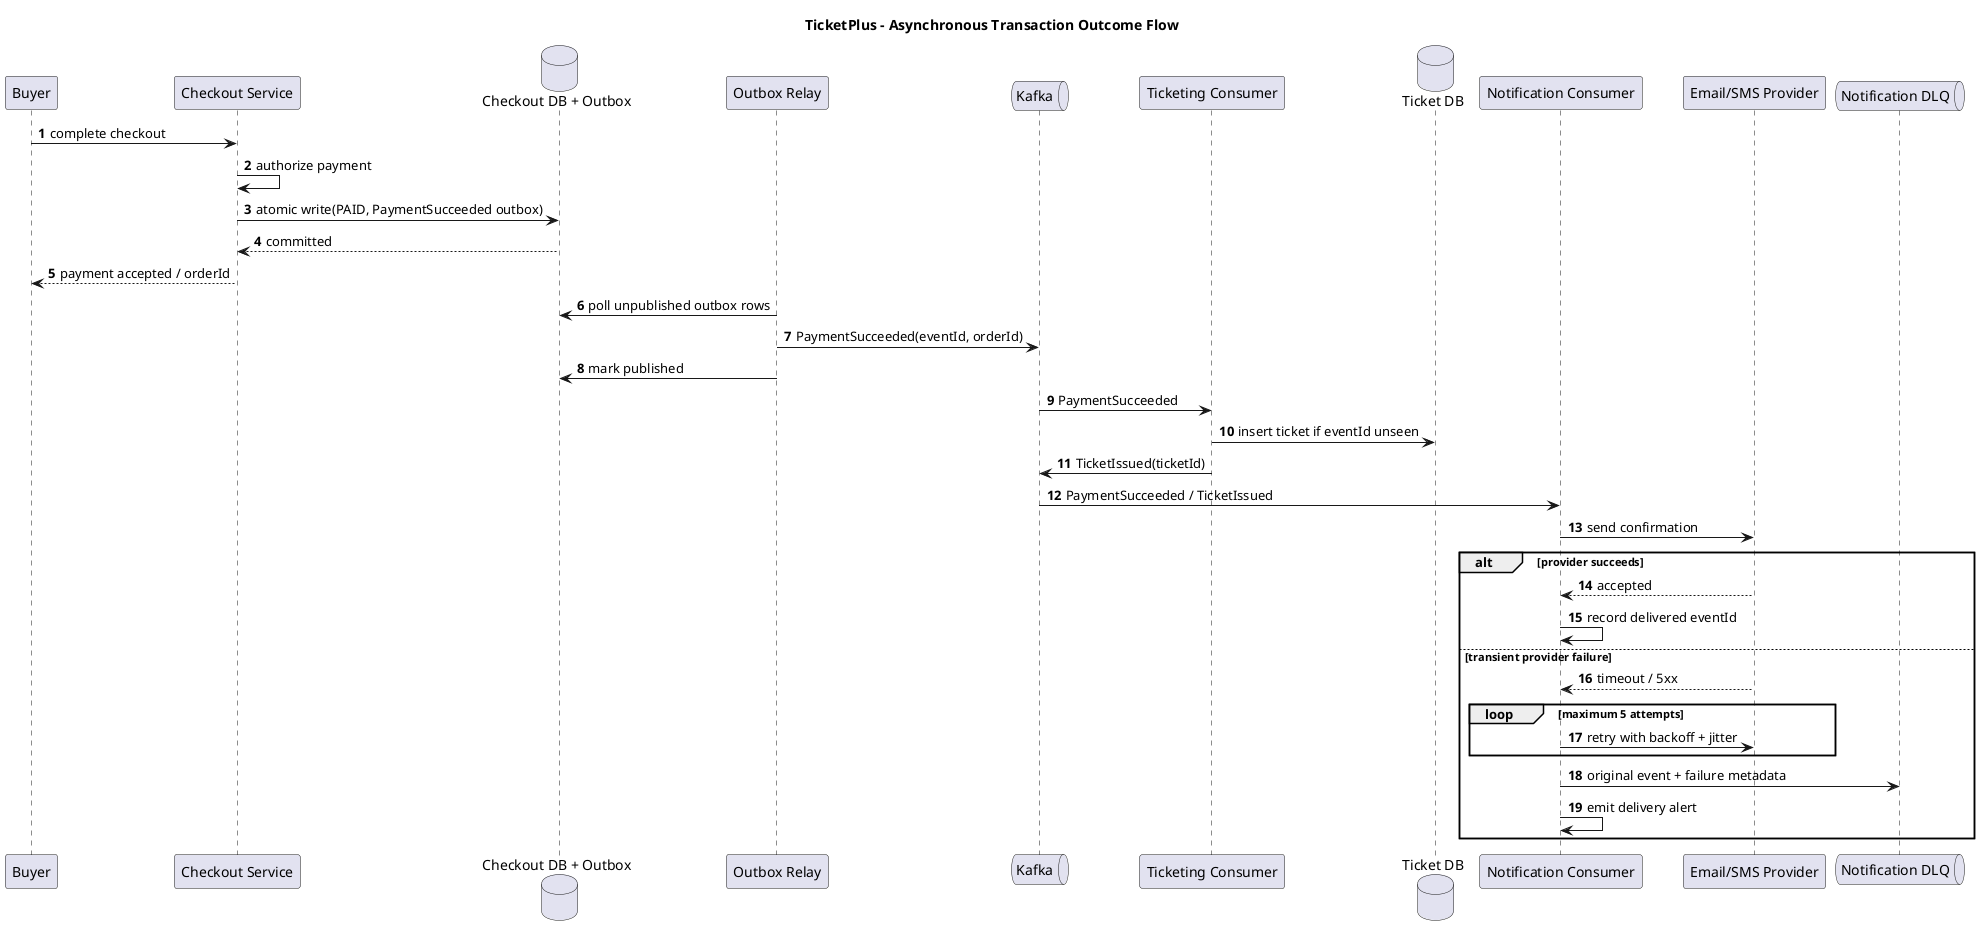
\includegraphics[width=0.96\textwidth,height=0.76\textheight,keepaspectratio]{figures/async-transaction-flow.png}
\caption{جریان غیرهم‌زمان نتیجه تراکنش}
\end{figure}

\subsection{پایش، SLO و انتشار Canary}
انتشار canary با ۵ درصد ترافیک آغاز و پس از پنجره‌های تحلیل به ۲۵، ۵۰ و ۱۰۰
درصد افزایش می‌یابد. عبور نرخ خطا، تأخیر یا conflict رزرو از نسخه پایدار، rollback
خودکار را فعال می‌کند. پرومتئوس معیارهای سرویس، ورودی، کوبرنتیز، کافکا، ردیس و
پستگرس را جمع و گرافانا نمایش می‌دهد. OpenTelemetry شناسه trace و correlation
را میان HTTP و پیام‌ها منتقل می‌کند.
\begin{figure}[H]
\centering
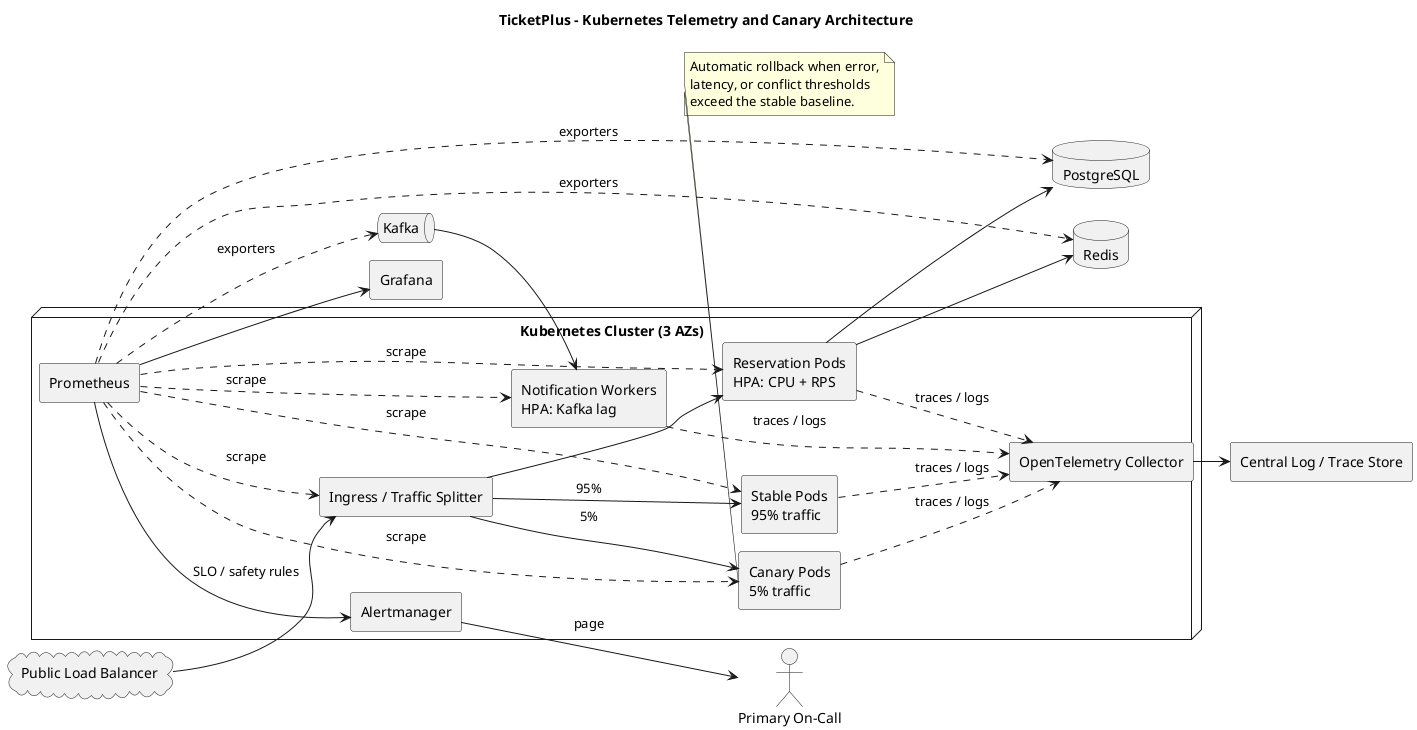
\includegraphics[width=0.96\textwidth,height=0.76\textheight,keepaspectratio]{figures/production-telemetry.png}
\caption{معماری مشاهده‌پذیری و انتشار Canary}
\end{figure}

اهداف اصلی شامل دسترس‌پذیری ۹۹٫۹۵ درصد برای قفل و پرداخت، صدک ۹۵ قفل کمتر از
۳۰۰ میلی‌ثانیه، lag کافکا کمتر از ۳۰ ثانیه و صفر رزرو مضاعف است. هر نشانه رزرو
مضاعف بلافاصله رخداد سطح یک ایجاد می‌کند.

\subsection{مدیریت رخداد}
شدت رخداد از \term{SEV-1} تا \term{SEV-4} تعریف شده است. فرمانده رخداد تصمیم و
اولویت، مسئول عملیات اقدام فنی، مسئول ارتباطات اطلاع‌رسانی و نویسنده timeline
را نگهداری می‌کند. on-call اولیه و ثانویه هفتگی هستند و عدم پاسخ در پنج دقیقه
به جانشین escalation می‌شود. پایان رخداد نیازمند پایداری SLO برای ۳۰ دقیقه،
تخلیه backlog و تطبیق رزرو، پرداخت و بلیت است.

\subsection{پسامورتوم‌های اجباری}
سه تحلیل بدون سرزنش تهیه شده است:
\begin{enumerate}
  \item خرابی درگاه پرداخت و باقی ماندن صندلی‌ها در حالت قفل؛ راه‌حل شامل circuit
  breaker، تطبیق با کلید تکرارپذیری و تأیید، آزادسازی یا قرنطینه سفارش است.
  \item شکست worker اتاق انتظار زیر بار شدید و پاسخ 503؛ راه‌حل شامل صف پایدار،
  حفظ توکن کاربر، حالت FIFO تنزل‌یافته و retry دارای jitter است.
  \item پارتیشن شبکه بین درگاه و رزرو؛ سامانه خرید را fail-closed می‌کند، policy
  معیوب را rollback و پس از بازیابی تطبیق انجام می‌دهد.
\end{enumerate}
هر پسامورتوم اثر، timeline، علت ریشه‌ای، عوامل تشدیدکننده، رفع و اقدام اصلاحی
دارای مالک و موعد را ثبت می‌کند.

\section{پیاده‌سازی مرجع و قراردادها}

\subsection{ساختار کد}
پیاده‌سازی مرجع در \en{src/ticketplus/} و با کتابخانه استاندارد پایتون ۳٫۱۳
نوشته شده است. هدف آن اثبات قواعد حیاتی بدون تحمیل وابستگی حجیم به محیط توسعه
است.
\begin{longtable}{P{4cm}P{10cm}}
\toprule
ماژول & مسئولیت\\
\midrule
\en{reservation.py} & تراکنش SQLite، قفل چندصندلی، انقضا، تأیید و آزادسازی\\
\en{checkout.py} & ساگای پرداخت، جبران، صدور بلیت و ثبت اعلان\\
\en{events.py} & گذرگاه رویداد محلی و مصرف تکرارناپذیر\\
\en{http_api.py} & آداپتور HTTP بدون وابستگی و endpointهای سلامت، رزرو، پرداخت و بلیت\\
\bottomrule
\end{longtable}

مهاجرت‌های پستگرس در \en{db/migrations/} schemaهای هویت، کاتالوگ، رزرو، پرداخت،
بلیت و اعلان را جدا می‌کنند. قید یکتایی مالک فعال در سطح دیتابیس نیز اعمال شده
است. جدول outbox برای انتشار پایدار رویدادها در نظر گرفته شده است.

\subsection{قرارداد API و رویداد}
فایل \en{contracts/openapi/ticketplus.yaml} قرارداد \term{OpenAPI 3.1} را برای
سلامت، ایجاد و دریافت رزرو، checkout و دریافت بلیت تعریف می‌کند. قراردادها
کلید Idempotency، ساختار مبلغ در واحد خرد و کدهای ۲۰۱، ۴۰۰، ۴۰۴ و ۴۰۹ را مشخص
می‌کنند. schemaهای JSON رویدادهای \term{PaymentSucceeded} و
\term{TicketIssued} شامل نسخه، شناسه aggregate، زمان و payload بدون داده کارت
هستند.

\subsection{اجرای محلی و بسته‌بندی}
فایل \en{Dockerfile} برنامه را با کاربر غیر root اجرا می‌کند. Compose پیش‌فرض
API مرجع و حجم پایدار SQLite را اجرا می‌کند. profile با نام
\en{production-parity} پستگرس، ردیس و کافکا را نیز بالا می‌آورد.

\begin{latin}
\begin{lstlisting}[language=bash]
docker compose up --build
curl http://localhost:8080/health/ready

docker compose --profile production-parity up --build

PYTHONPATH=src python3 -m unittest discover -s tests -v
python3 quality/coverage/run.py
python3 quality/mutation/run.py
\end{lstlisting}
\end{latin}

اسکریپت \en{scripts/package-submission.sh} فایل ZIP را بدون metadata گیت، state
ترافورم، cache و bytecode می‌سازد. صحت استخراج آرشیو آزمایشی نیز بررسی شد.

\section{استانداردهای مهندسی و نقش‌های تیم}

هر سرویس تولیدی باید dependency قفل‌شده، container چندمرحله‌ای، endpointهای
سلامت، log ساختاریافته، معیار پرومتئوس، قرارداد نسخه‌دار، مهاجرت سازگار، آزمون
و runbook داشته باشد. داده کارت ذخیره نمی‌شود و secret در مخزن یا log قرار
نمی‌گیرد. تغییر قرارداد شکستن‌پذیر نیازمند نسخه جدید و بازه مهاجرت است.

دیدگاه‌های شبیه‌سازی‌شده شامل مالک محصول، تحلیلگر سیستم، توسعه‌دهنده backend و
frontend، متخصص QA، مهندس DevOps/SRE، بازبین امنیت و فرمانده رخداد است. ماتریس
مسئولیت، شخص پاسخگو، مشاوران و افراد مطلع را برای محدوده، قرارداد، رزرو، پرداخت،
آزمون، زیرساخت، رخداد و انتشار مشخص می‌کند.

برای دفاع معماری، اعضا باید بتوانند تصمیم مالکیت موجودی، ترکیب ردیس و قید
دیتابیس، انتخاب ساگا به جای تراکنش توزیع‌شده، سازگاری نهایی جست‌وجو، تحویل
حداقل یک‌بار کافکا، انتشار canary، نتیجه آزمون رقابتی و محدودیت تک‌منطقه‌ای را
توضیح دهند.

\section{موارد باقی‌مانده برای نسخه تحویلی گروه}

بخش‌های زیر عمداً توسط این گزارش جعل یا تکمیل فرض نشده‌اند و باید با شواهد
واقعی گروه جایگزین شوند:

\begin{enumerate}
  \item سند نهایی چشم‌انداز محصول؛
  \item سند نهایی تحلیل و کاهش ریسک؛
  \item خروجی کامل جیرا، نمودارهای burndown، review و retrospective؛
  \item نام، شماره دانشجویی و تقسیم کار واقعی اعضا؛
  \item تصاویر pipeline واقعی گیت‌لب و merge requestها؛
  \item نتیجه اجرای k6 در محیط تست استقرار‌یافته؛
  \item نتیجه نهایی \en{terraform validate} در CI با provider قابل دسترس؛
  \item تاریخ ارائه، لینک مخزن و شناسه commit نهایی.
\end{enumerate}

\reservedbox{محل درج شواهد نهایی}{پس از آماده شدن موارد بالا، این کادر با
جدول یا فهرست دقیق فایل‌ها، لینک‌ها، تصاویر و شناسه commit نسخه تحویلی جایگزین
شود.}

\section{جمع‌بندی}

معماری تیکت‌پلاس مسئله فروش بلیت پرترافیک را با تفکیک روشن مالکیت داده، کنترل
هم‌زمانی در رزرو، ساگای پرداخت، صدور مستقل بلیت، پیام‌رسانی مقاوم و مشاهده‌پذیری
تولید حل می‌کند. نمودارهای UML، ترافورم، قراردادهای API و رویداد، مهاجرت‌های
داده، محیط container، خط لوله CI و اسناد عملیات از یک مدل واحد پیروی می‌کنند.
پیاده‌سازی و آزمون مرجع نشان می‌دهد قاعده حیاتی مالکیت یکتای صندلی در رقابت
هم‌زمان حفظ می‌شود و آزمون‌ها نسبت به خطاهای هدفمند حساس هستند. با افزودن اسناد
چشم‌انداز و ریسک و خروجی واقعی جیرا توسط گروه، بسته نهایی همه اقلام مورد انتظار
شرح پروژه را در قالبی منسجم و قابل دفاع پوشش خواهد داد.

\appendix
\section{فهرست مسیرهای مهم مخزن}
\begin{latin}
\begin{lstlisting}
diagrams/                              UML sources
rendered/                              baseline SVG exports
docs/architecture-and-operations/     DDD, messaging, telemetry, incidents
docs/quality/                         QA, load, coverage, mutation policies
docs/project-governance/              roles, standards, defense guide
src/ticketplus/                       executable reference implementation
tests/                                unit, concurrency, HTTP tests
contracts/                            OpenAPI and event schemas
db/migrations/                        PostgreSQL schema and seed
infra/terraform/                      AWS infrastructure as code
quality/load/                         k6 contention scenario
quality/coverage/                     coverage runner
quality/mutation/                     mutation runner
scripts/package-submission.sh         reproducible ZIP packaging
\end{lstlisting}
\end{latin}

\section{پیوست‌های رزروشده}
\reservedbox{پیوست الف: چشم‌انداز و تحلیل ریسک}{نسخه‌های نهایی یا ارجاع دقیق
به فایل‌های مستقل در بسته تحویل درج شود.}
\reservedbox{پیوست ب: شواهد جیرا}{خروجی backlog، sprint، burndown، review و
retrospective درج شود.}
\reservedbox{پیوست پ: شواهد CI و آزمون بار}{تصاویر pipeline، گزارش k6 و شناسه
commit نهایی درج شود.}

\end{document}
